\section{Calculating susceptibility}
    \label{Sec:Exp:Susceptibility}

Code to calculate the Lindhard susceptibility was written in MATLAB \footnote{Full code is found in appendix \ref{Appendix:SusceptibilityCode}} and early versions were tested with free electron cases in 2 and 3 dimensions with results shown in figure~\ref{Fig:Exp:FreeElectronSusceptibility}. This matches the expected free electron curves\footnote{See, for example, page 126 and Appendix F of reference\cite{Dressel2002}}. One caveat when dealing with the free electron case is that the energy dispersion is not periodic and as such needs to be truncated at some point in a spherically symmetric way. This truncation affects the final calculation but provided it occurs far enough from the Fermi surface then the difference is minimal. The results shown are for a calculated region that was a sphere of radius 1 with a Fermi surface radius of 0.3. Values for $\delta$(=1e-9) and $\omega$(=1e-9) are somewhat arbitrary given that the dispersion is simplified with $\hbar^2/2m = 1$ but are given here for posterity. 

\begin{figure}[htbp]
    \begin{center}
        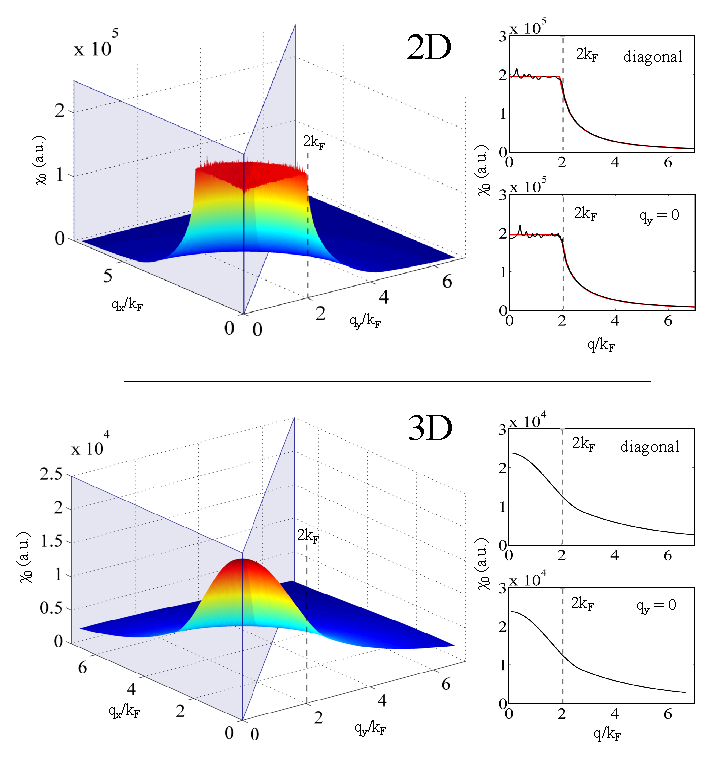
\includegraphics[scale=0.9]{Chapter-ExperimentalTechnique/Figures/Susceptibility/FreeElectron/FreeElectron}
        \caption{The real part of the Lindhard susceptibility calculations for a free electron model at \unit{T=0}{\kelvin} using the MATLAB \code{calc_x0.m} code. Top panels are for the 2D case over a $500\times500$ point grid, the bottom panels are for the 3D case taken over a $100\times100\times100$ point grid. Panels to the right correspond to slices through the surface plots on the left. Calculations in the 3D case are at $q_z=0$.}
        \label{Fig:Exp:FreeElectronSusceptibility}
    \end{center}
\end{figure}


The code was adapted to accept pre-generated energy dispersions as calculated with the WIEN2k DFT software and post-processed with Ed's MATLAB code. In this case, the dispersion is periodic and energies at the scattering vector $q$ are obtained by simply `rolling' the 3D matrix of energy values. Testing on this adapted code was performed by re-creating WIEN2k calculations on LaFeAsO$_{0.1}$F$_{0.9}$ performed by Mazin et al.\cite{Mazin2008} and then comparing our own susceptibility calculations with those in the Mazin paper. A temperature smearing of \unit{1}{\milli Ry} was quoted which was equated, using the Boltzman conversion, to a temperature of \unit{157.88}{\kelvin}. A similar amount of points ($55\times55\times26$) was also used.

Figure~\ref{Fig:Exp:MazinX0Comparison} show comparisons of $\Real \chi_0(q,\omega)$ and $\Imag \chi_0(q,\omega)$ with the published results. For these calculations the values of $\delta=\textrm{1e-4}$ and $\omega=\textrm{1e-6}$ were determined to give the closest results from a series of trials\footnote{There is no indication in the paper as to the values of $\delta$ and $\omega$ used in their own calculations although we know that they are likely to be of the order of the temperature energy scale (\unit{1}{\milli Ry}) or less.}. The comparison shows that some of the finer structure from the Mazin paper is missing from our own calculations, for example the depression in the real part at the $\Gamma$ point, however the overall shape is very similar.

\begin{figure}[htbp]
    \begin{center}
        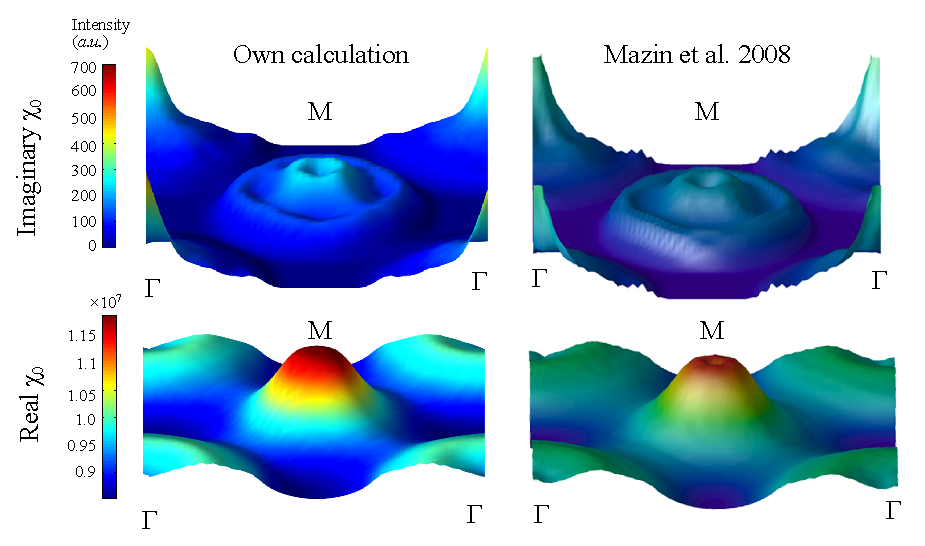
\includegraphics[scale=0.9]{Chapter-ExperimentalTechnique/Figures/Susceptibility/MazinComparison/MazinComparison}
        \caption{Right hand panels show the real and imaginary parts of Lindhard susceptibility calculations on LaFeAsO$_{0.1}$F$_{0.9}$ by Mazin et al. for $q_z=\pi/c$, right panels show the same calculation performed using our own MATLAB code.}
        \label{Fig:Exp:MazinX0Comparison}
    \end{center}
\end{figure}


The Lindhard function is very sensitive close to the Fermi surface and finite sampling of the energy data  can cause imperfect cancellation in the calculation --- particularly in the imaginary part. Applying a temperature smearing to the function is useful to gloss over the finite element size in the calculation which can cause significant spikes in the results. Figure~\ref{Fig:Exp:SusceptibilityTempSmearing} shows the smearing at a series of temperatures and that a temperature of \unit{158}{\kelvin} corresponds approximately to a smearing over 2 grid intervals at the Fermi surface. An appropriate choice of temperature depends on the granularity of your model as well as the expected fine detail of the results. The Mazin investigation was into a similar quasi two-dimensional pnictide material that used a comparable number of data points and so we also opted to use \unit{158}{\kelvin} for the temperature smearing.

Smearing also occurs when a finite quasi-particle lifetime, $\delta$, is factored in and when the perturbing field is oscillatory with frequency, $\omega$. These values are also not known \textit{a priori} and so we again look to the energy scale of the spacing between grid points close to the Fermi surface for guidance.

\begin{figure}[htbp]
    \begin{center}
        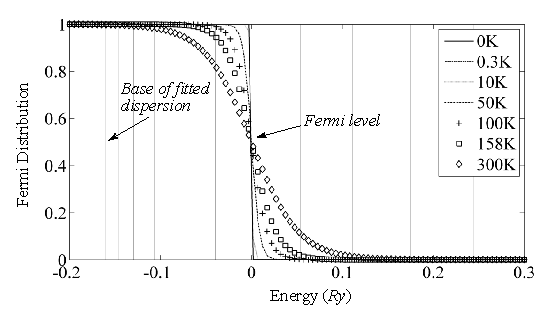
\includegraphics[scale=0.9]{Chapter-ExperimentalTechnique/Figures/Susceptibility/TempSmearing/TempSmearing}
        \caption{The Fermi distribution plotted at various temperatures. Vertical lines represent typical grid energy spacings for a free electron distribution fitted to a portion of bandstructure for LaFeAsO$_{01}$F$_{0.9}$ which rounds out just below the Fermi surface. We can see that for \unit{158}{\kelvin}, the smearing spans approximately 2 grid intervals at the Fermi energy.}
        \label{Fig:Exp:SusceptibilityTempSmearing}
    \end{center}
\end{figure}

